%!TEX root = ../main.tex

\chapter{Numerical Experiments}

In this section we describe the implementation of the algorithm. We also compare its performance with different alternative methods.

\section{Implementation details}

In this section we describe the implementation of the algorithm described in the previous chapter. But before anything else, we remind the reader the problem setting and the estimator considered. 
\subsection{Problem considered}
We observe $n$ independent random vectors $\bX_1,\ldots,\bX_n\in\calX$ drawn from a probability distribution $P^*$ that admits a density function $f^*$. Given a family of mixture components $f_1,\ldots,f_K$, we assumed that this unknown density is well approximated by a convex combination $f_{\bpi}$ of these components
\begin{equation}
f_{\bpi}(\bx)=\sum_{j=1}^K\pi_j f_j(\bx), \quad \bpi \in \BB_+^K=\Big\{\bpi\in [0,1]^K: \sum_{j=1}^K\pi_j=1\Big\}.
\end{equation}
The component densities $\calF=\{f_j:j\in[K]\}$ are assumed to be given by previous experiments or expert knowledge. The problem of construction of this family is an open problem that we try to address in section ?. Our objective is to estimate the weight vector $\bpi$ from the simplex $\BB_+^K$ under the sparsity scenario and investigate the statistical properties of the Maximum Likelihood Estimator (MLE), defined by
\begin{equation}
\label{MLE_2}
\hat\bpi \in \argmin_{\bpi\in \Pi}\big\{-\frac{1}{n}\sum_{i=1}^n\log f_{\bpi}(\bX_i)\big\},
\end{equation}
where the minimum is computed over a suitably chosen subset $\Pi$ of $\BB_+^K$. 
\subsection{Implementation}
The computation of \cref{MLE_2} is fairly simple as the objective function and the set $\Pi$ are convex and can be easily solved by convex programming. We wrote the algorithm in Python and used the modeling language CVXPY\cite{cvxpy}.\\
We give a dictionary of densities in input.\\
Give pseudo code
\begin{python}
from sklearn.base import BaseEstimator
import numpy as np
from cvxpy import *


class WeightEstimator(BaseEstimator):

    def __init__(self, densities_dict, select_threshold=10e-3):
        self.densities_dict  = densities_dict
        self.K = len(self.densities_dict)
        self.select_threshold = select_threshold

    def fit(self, X):
        self.F = np.array([self.densities_dict[i].pdf(X) for i in range(self.K)]).T
        F = np.array([self.densities_dict[i].pdf(X) for i in range(self.K)]).T
        self.pi = Variable(self.K)
        constraints = [sum_entries(self.pi) == 1, self.pi >= 0, self.pi <= 1]
        objective = Minimize(-sum_entries(log(F * self.pi)))
        prob = Problem(objective, constraints)
        prob.solve()
\end{python}

\section{Alternative methods considered}
\subsection{SPADES}
From \cite{SPADES}
\subsection{Adaptive Dantzig density estimation}

We will compare our method with the Adaptive Dantzig estimator in the density model which has been introduced in \cite{Bertin}. This method is similar to ours as it construct an estimator of the unknown density from a linear mixtures of functions taken from a dictionary. The key idea of this paper is to minimize the $\ell_1$-norm of the weight vector of the linear combination under an adaptive Dantzig constraint. This constraint comes from sharp concentration inequalities. We recall here some material about the Dantzig selector. It has been introduced by \cite{candes2007} in the linear regression model
\begin{equation}
	Y = A\lambda_0 + \epsilon
\end{equation}
where $Y\in \RR^n$, $A$ is a $n$ by $M$ matrix, $\epsilon \in \RR^n$ is the noise vector and $\lambda_0$ the unknown regression parameter to estimate. The Dantzig estimator is then defined by\todos{Définir $\ell_1$ et $\ell_{\infty}$}
\begin{equation}
	\hat\lambda^D = \argmin{\lambda \in \RR^M} \|\lambda \|_1 \quad \text{subject to} \quad \| A^T(A\lambda-Y)\|_{\infty} \leq \eta.
\end{equation}
where $\eta$ is the regularization parameter. \cite{bickel2009} considered the non-parametric regression framework
\begin{equation}
		Y_i = f(x_i) + e_i, \quad i=1,\dots,n
\end{equation}
where $f$ is an unknown function, the design points $(x_i)_{i=1,\dots,n}$ are known and $(e_i)_{i=1,\dots,n}$ is a noise vector. One can estimate $f$ as a weighted sum $f_{\lambda}$ of elements of a dictionary $D=(\varphi_m)_{m=1,\dots,M}$
\begin{equation}
\label{linear_mix_density}
	f_{\lambda} = \sum_{i=1}^M\lambda_m\varphi_m.
\end{equation}
 The goal of \cite{Bertin} was to estimate an unknown density $f_0$ with respect to a known measure $dx$ on $\RR$ by using the observation of $n$-sample $X_1,\dots,X_n$ and build a linear mixture density $f_{\lambda}$ of elements of the dictionary $D$ as in \cref{linear_mix_density}. Let us consider the empirical scalar product of $f_0$ and $\varphi_m$
\begin{equation}
    \hat\beta_m = \frac{1}{n}\sum_{i=1}^n\varphi_m(X_i) \xrightarrow{\text{a.s}} \int \varphi_m(x)f_0(x)dx=\beta_{0,m},
\end{equation}
and the Gram matrix associated to the dictionary $D$
\begin{equation}
    G_{m,m'}=\int\varphi_m(x)\varphi_{m'}(x)dx \quad \text{with}\quad 1\leq m,m' \leq M.
\end{equation}
The scalar product of $f_{\lambda}$ and $\varphi_m$ is therefore
\begin{equation}
    \int\varphi_m(x)f_{\lambda}(x)dx = \sum_{m'=1}^M\lambda_{m'}\int\varphi_{m'}(x)\varphi_m(x)dx = (G\lambda)_m.
\end{equation}
The Dantzig estimate $\hat\lambda^D$ is then obtained by solving the following constrained minimization problem
\begin{equation*}
    \left\{
    \begin{array}{ll}
        \text{minimize}\, &\|\lambda\|_1 \\
        \text{subject to}\, &|(G\lambda)_m-\hat\beta|\leq \eta_{\gamma,m} \quad m\in \{1,\dots,M\},
    \end{array} \right.
\end{equation*}
where for a constant $\gamma > 0$ chosen 
\begin{equation}
    \eta_{\gamma,m} = \sqrt{\frac{2\tilde\sigma_m^2\gamma\log{M}}{n}}+ \frac{2\|\varphi_m\|_{\infty}\gamma\log{M}}{3n},
\end{equation}
with
\begin{equation}
    \tilde\sigma_m^2 = \hat\sigma_m^2+2\|\varphi_m \|_{\infty}\sqrt{\frac{2\hat\sigma_m^2\gamma\log{M}}{n}}+ \frac{8\|\varphi_m\|_{\infty}^2\gamma\log{M}}{n},
\end{equation}
and
\begin{equation}
    \hat\sigma^2_m = \frac{1}{n(n-1)}\sum_{i=2}^n\sum_{j=1}^{i-1}(\varphi_m(X_i)-\varphi_m(X_j)).
\end{equation}
Note that $\eta_{\gamma,m}$ depends on the data which explains the name \textit{Adaptive Dantzig}. The authors of \cite{Bertin} derived the form of $\eta_{\gamma,m}$ from sharp concentration inequalities (see theorem 1 of \cite{Bertin}). More precisely, if we consider $\lambda_0=(\lambda_{0,m})_{m=1,\dots,M}$ such that the projection of $f_0$ on the space spanned by $D$ is
\begin{equation}
    \textbf{P}_{D}f_0=\sum_{m=1}^M\lambda_{0,m}\varphi_m,
\end{equation}
then $(G\lambda_0)_m=\beta_{0,m}$ \todos{a expliquer} and the parameter $\eta_{\gamma,m}$ can be seen as the smallest quantity such that, for $\gamma > 1$, we have $|\beta_{0,m}-\hat\beta_m|\leq \eta_{\gamma,m}$ with high probability. The main result of this paper is a bound on the $L_2$ risk of the adaptive Dantzig density estimator with high probability without any assumptions on the unknown density $f_0$ \todos{parler des hypotheses sur la matrice Gram}. The discussion of this result goes beyond the scope of this section. Note that the assumption $\gamma > 1$ is an almost necessary condition to have a theoretical control on the quadratic error $\Ex\|\hat f^D-f_0 \|^2_2$. Therefore, we will follow the choice of $\gamma=1.01$ made by the authors in our experiments. The pseudo code of the procedure is given in \cref{algo:ad_algo}. 

\begin{figure}[H]
\begin{center}
\mybox{
\begin{minipage}{0.85\linewidth}
\begin{algorithmic}[1]
\small
\STATE {\bfseries Input:} A sample $\bX_1,\ldots,\bX_n\in\RR^p$ and the dictionary $D=(\varphi_m)_{m=1,\dots,M}$.
\STATE {\bfseries Output:} Dantzig estimate $\hat \lambda^D$.
\STATE {\bfseries Init:} Set $\gamma=1.01$.
\STATE Compute $\hat\beta_m = \frac{1}{n}\sum_{i=1}^N\varphi_m(X_i)$.
\STATE Compute $\hat\sigma^2_m = \frac{1}{n(n-1)}\sum_{i=2}^n\sum_{j=1}^{i-1}(\varphi_m(X_i)-\varphi_m(X_j))^2$.
\STATE Compute $\tilde\sigma_m^2$.
\begin{equation}
    \tilde\sigma_m^2 = \hat\sigma_m^2+2\|\varphi_m\|_{\infty}\sqrt{\frac{2\hat\sigma_m^2\gamma\log{M}}{n}}+ \frac{8\|\varphi_m\|_{\infty}^2\gamma\log{M}}{n}.
\end{equation}
\STATE Compute $\eta_{\gamma,m}$
\begin{equation*}
    \eta_{\gamma,m} = \sqrt{\frac{2\tilde\sigma_m^2\gamma\log{M}}{n}}+ \frac{2\|\varphi_m\|_{\infty}\gamma\log{M}}{3n}.
\end{equation*}
\STATE Compute the coefficients $\hat\lambda^{D,\gamma}$ of the Dantzig estimate, $\hat\lambda^{D,\gamma}=\argmin_{\lambda\in\RR^M}\|\lambda \|_1$ such that $\lambda$ satisfies the Dantzig constraint
\begin{equation}
    \forall m \in \{1,\dots,m\}, \quad |(G\lambda)_m-\hat\beta_m|\leq \eta_{\gamma,m}.
\end{equation}

\end{algorithmic}
\end{minipage}
}
   \caption{Adaptive Dantzig density estimation procedure}
   \label{algo:ad_algo}
\end{center}
\vspace{-15pt}
\end{figure}


\subsection{Kernel density estimation}

The kernel density estimator is a well established non-parametric way of estimating the probability density function of a random variable. We will recall in this section some material about KDE.\\
Let $X_1,\dots,X_n$ be i.i.d random variables drawn from an unknown probability density $f$ with respect to the Lebesgue measure on $\RR$. The kernel density estimator $\hat f_h $ is given by
\begin{equation}
	\hat f_h(x) \triangleq \frac{1}{n}\sum_{i=1}^nK\Big(\frac{X_i-x}{h}\Big)
\end{equation}
where $K:\RR \rightarrow \RR$ and $\int K(u)du = 1$ is called a Kernel and $h$ is the bandwidth. We used gaussian kernels and the Sheather and Jones bandwidth selection procedure (\cite{sheather_bdwth}) described below

\section{Experimental Evaluations}

In the experimental evaluation, we had to construct a set of target densities with different shapes to evaluate the performances of the estimators. We also had to build different density (more generally functions) dictionaries. Finally we assessed the performance through the Kullback-Leibler and $L_2$ distance.

\subsection{Dictionaries considered}
\begin{enumerate}
\item Gaussians
\item A union of Gaussians and Laplacians densities called $D$. The Gaussians has their means in $[0, 0.2, 0.4, 0.6, 0.8, 1]$ and their variances in $[0.001, 0.01, 0.1, 1]$. The Laplacians has their means in $[0.05, 0.1, 0.5, 1]$ and their scales in $[0, 0.2, 0.4, 0.6, 0.8, 1]$. Therefore $D$ has 48 elements.

\begin{figure}
\centering
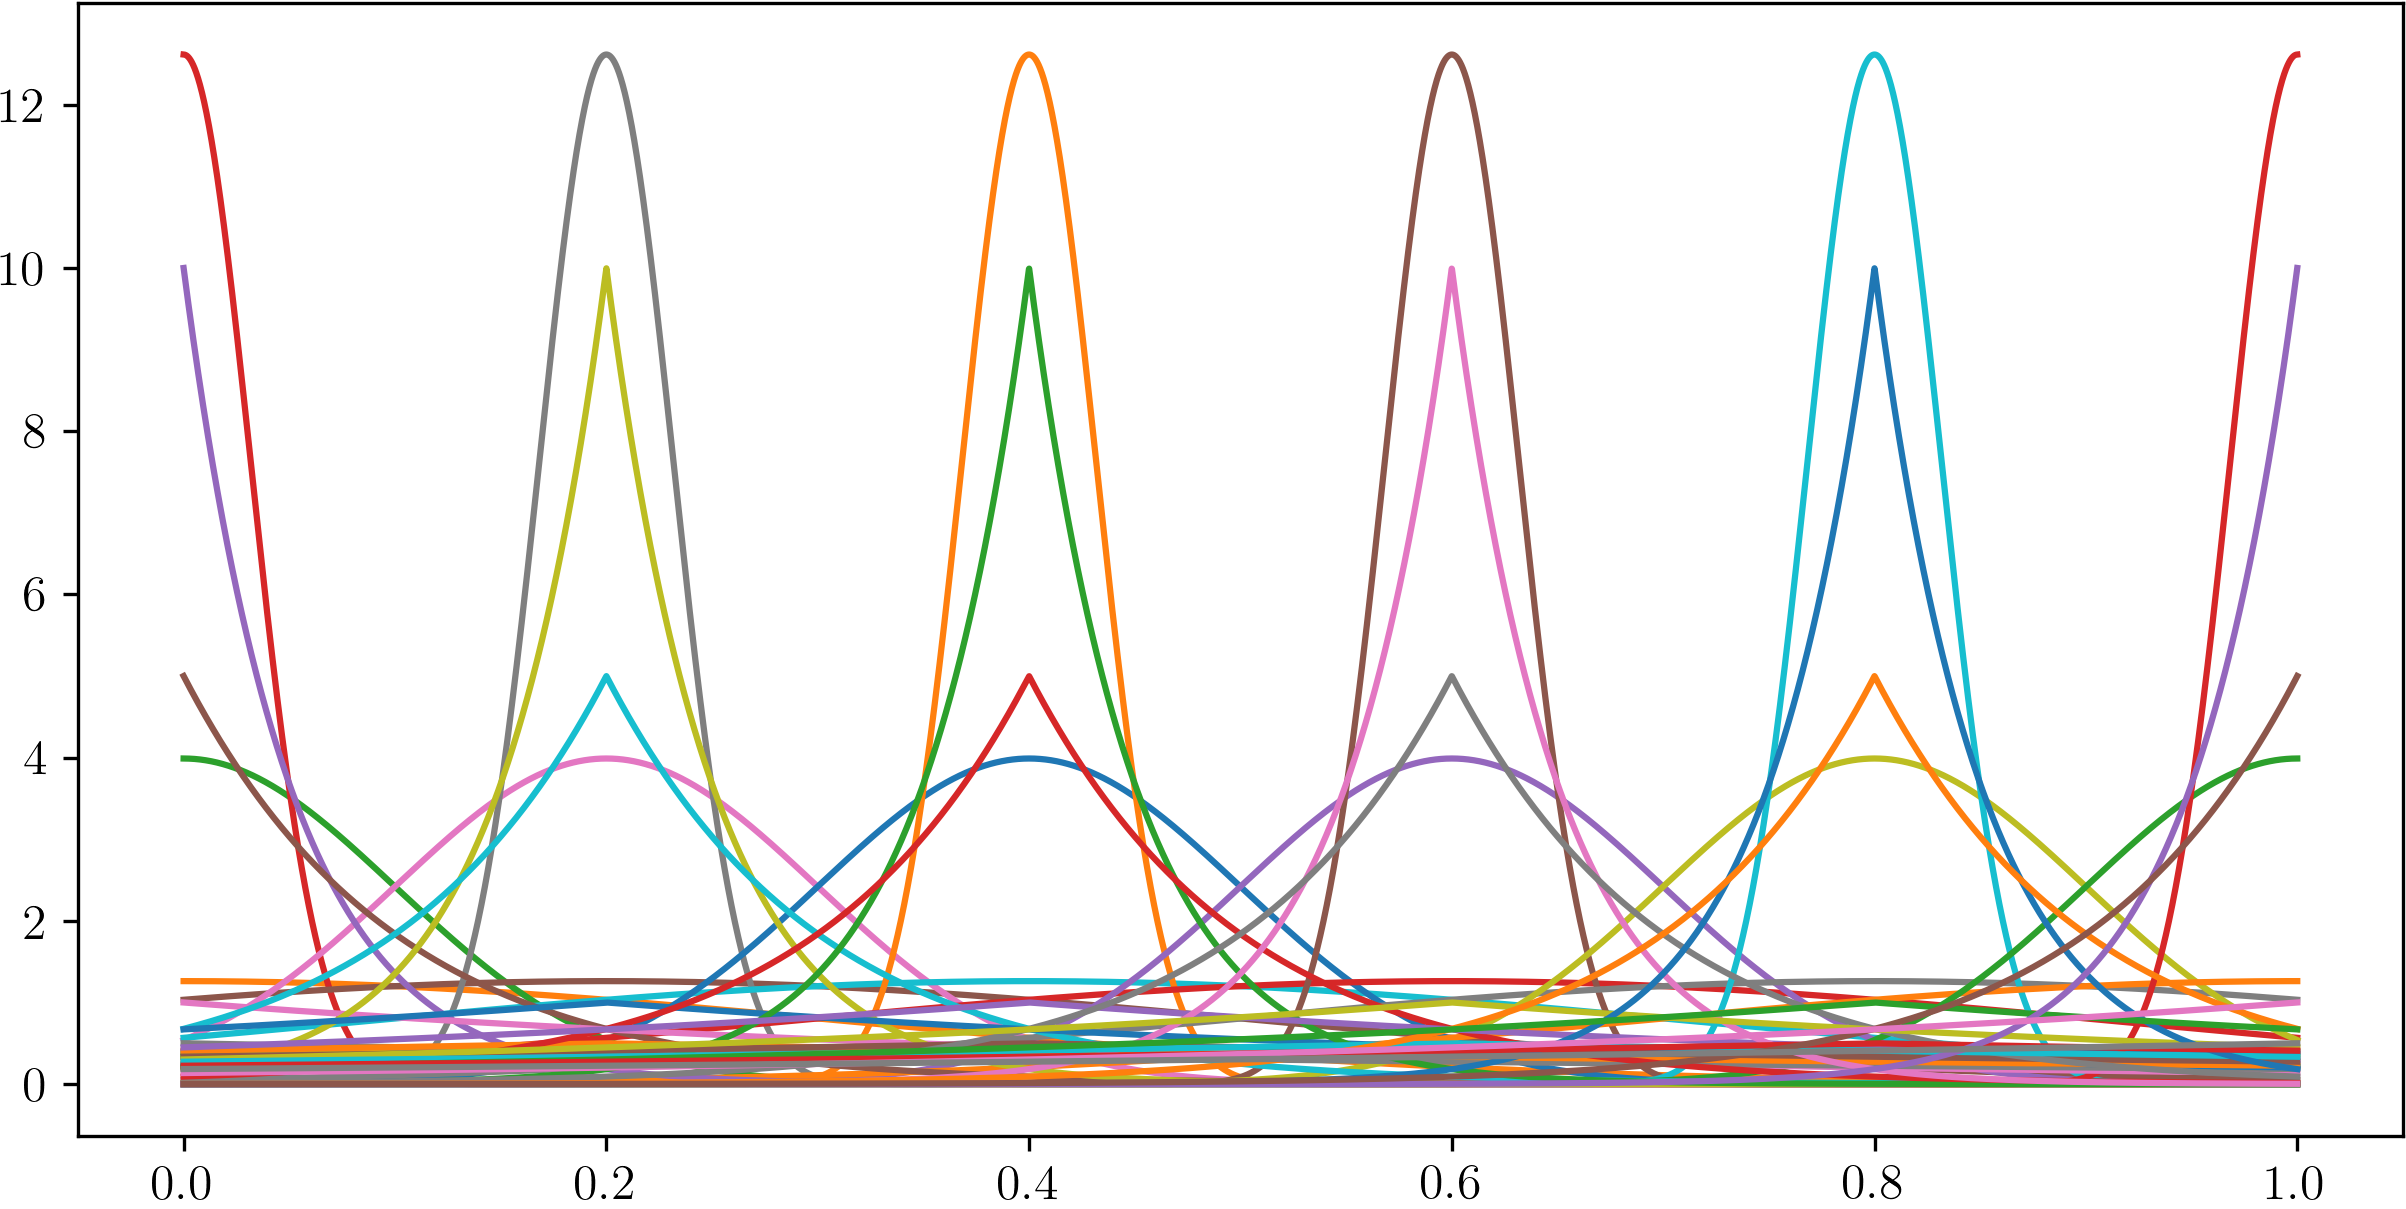
\includegraphics[width=1\textwidth]{TeX_files/lapl_gauss_dict.png}
\caption{Union of Gaussians and Laplacians,}
\end{figure}
\item Haar wavelet basis ?
\item Daubechies wavelet ?
\item Union of Fourier and Haar aud Gaussians ?
\end{enumerate}

\subsection{Densities considered}
We considered 5 target densities
\begin{enumerate}
\item[$f_{unif}$:] A uniform on $[0,1]$ 
\item[$f_{rect}$:] A mix of uniform densities on subintervals called "Rectangular":
\begin{equation}
    f_{rect}(x)=\frac{10}{7}\b1_{[0,1/5]}+\frac{5}{7}\b1_{[1/5,2/5]}+
    \frac{10}{7}\b1_{[2/5,3/5]}+\frac{10}{7}\b1_{[4/5,1]}
\end{equation}
\item[$f_{gauss}$:] A mixture of 5 Gaussian densities taken from the dictionary $D$ equally reparted in $[0,1]$.\todos{A retravailler}
\begin{equation}
    f_{gauss}(x)=\sum_{k=1}^5 0.2f_{\pi(k)}(x) \quad \text{with}\quad f_k\in D
\end{equation}

\item[$f_{gauss-lapl}$:] A mix of Gaussian and Laplacian densities taken from the dictionary (donner un nom au dictionaire $D$)
\begin{equation}
    f_{gauss-lapl}(x)=\sum_{k=1}^5 0.2f_{k}(x) \quad \text{with}\quad f_k\in D
\end{equation}
\item[$f_{ext}$:] A mixture of Gaussian and Laplacian densities  taken from another dictionary $D_{out}$
\begin{equation}
    f_{ext}(x)=\sum_{k=1}^7 \frac{1}{7}f_{k}(x) \quad \text{with}\quad f_k\in D_{out}
\end{equation}
\end{enumerate}
These target densities are plotted in \cref{fig:target_densities}.
\begin{figure}
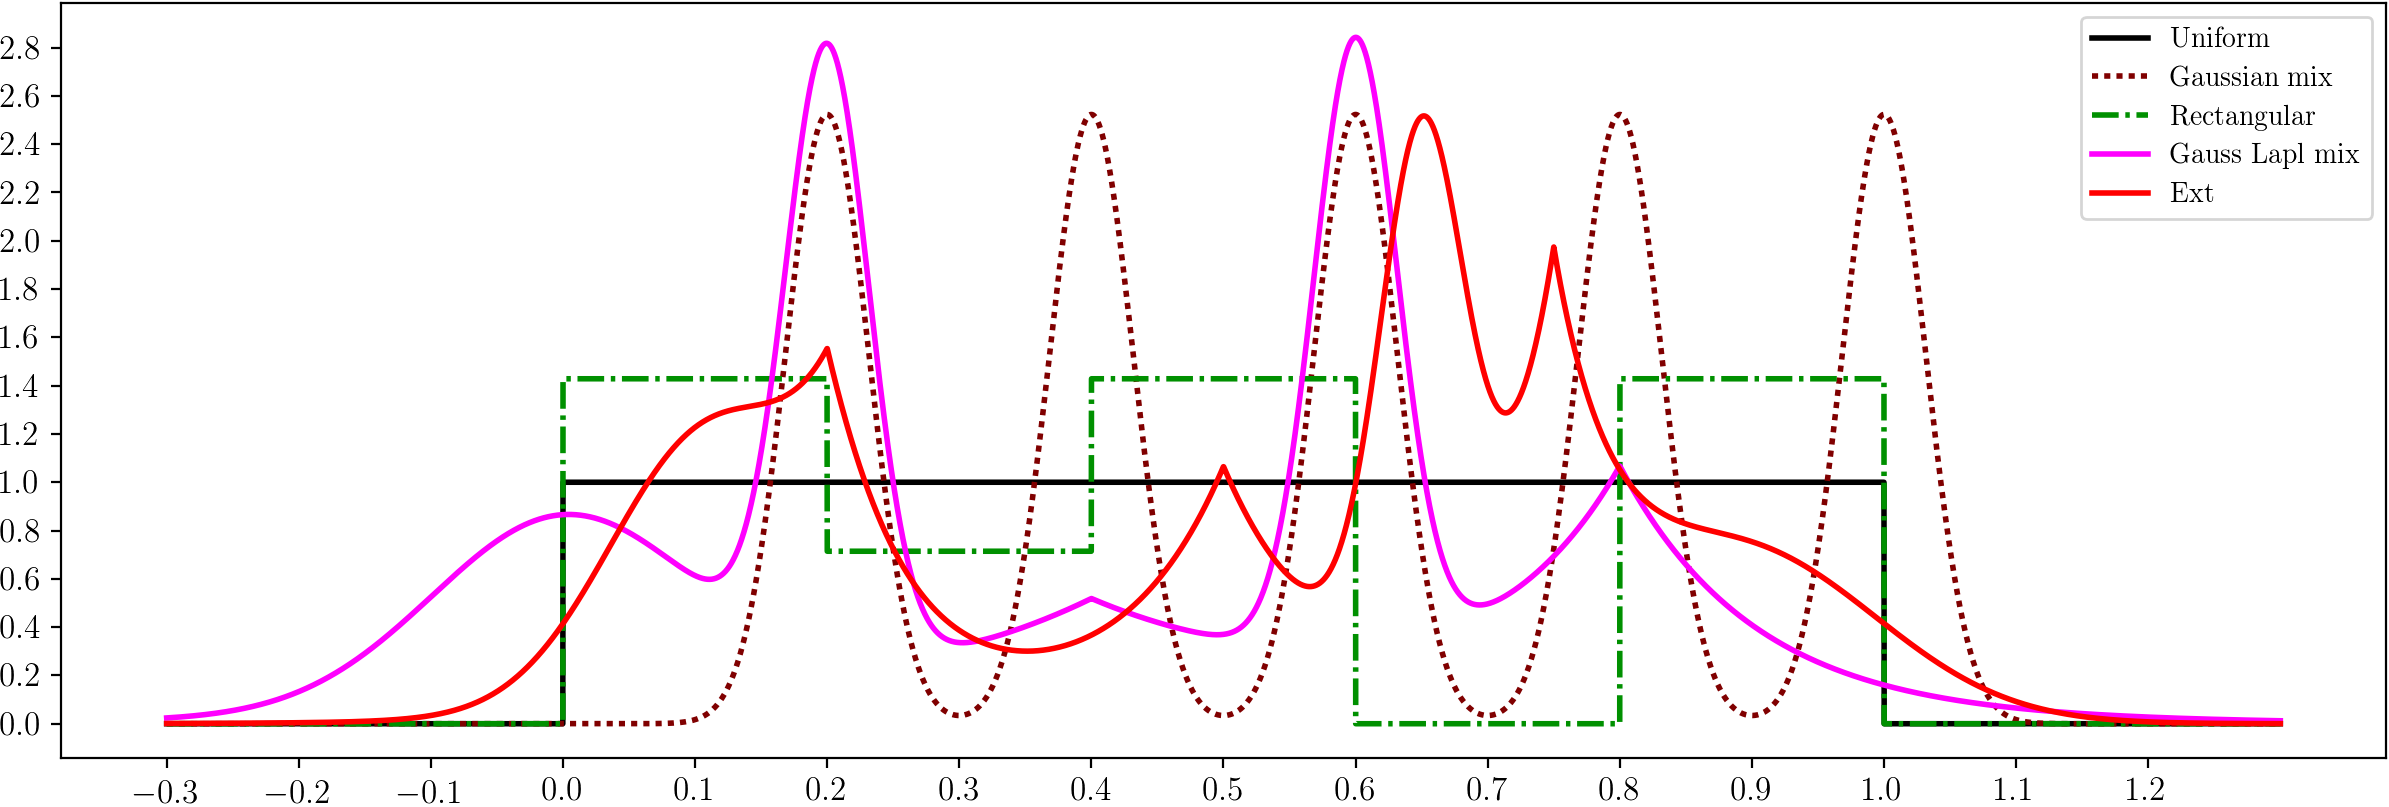
\includegraphics[width=1.2\textwidth]{TeX_files/densities_f_star.png}
\caption{Five target densities considered.}
\label{fig:target_densities}
\end{figure}

\subsection{Results}
The results are ploted in \cref{fig:full_res}. The dictionary used for the Adaptive Dantzig and the Maximum Likelihood estimator is $D$. At first glance, the performance of the MLE seems good in Kullback-Leibler loss and $L_2$. The method showing the worst performance in all scenarios is the Adaptive Dantzig. Note that it is interesting to compare the MLE to A.D as both methods relies on a dictionary. the MLE present a relative small variance, lesser than the Kernel density estimator with the Sheather-Jones bandwidth selector which is the best KDE method studied regarding the loss. Another interesting observation is the small impact of the size of sample for the MLE. We will cover each scenarios. Unsurprisingly the MLE does not perform as well as kernel based methods on the uniform case as the dictionary given could not provide a good mixture density that approach well this target density. This goes as well for the rectangular density $f_{rect}$ which shows the worst performance for the MLE. It should be possible to increase the performance of the MLE by adding uniform on different segments of $[0,1]$.
\begin{figure}
    \hspace{-2cm}
    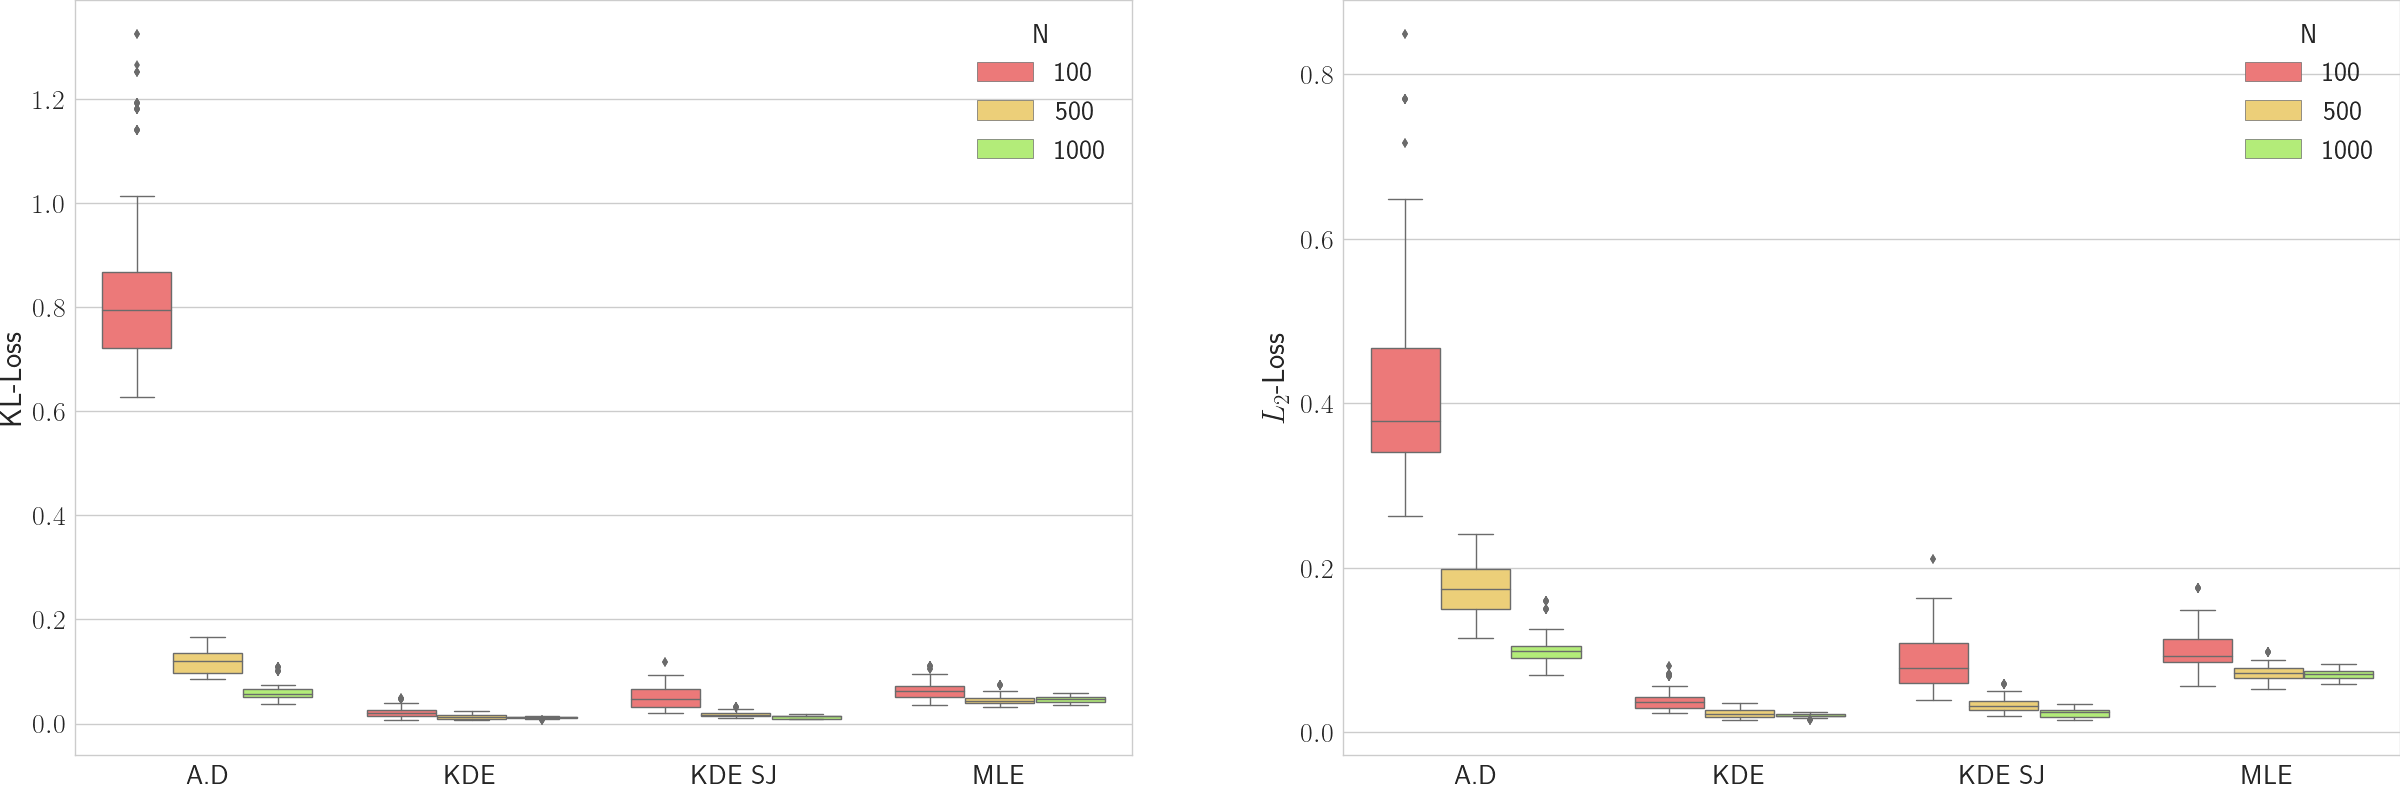
\includegraphics[width=1.2\textwidth]{./TeX_files/full_results.png}
    \caption{Results of Adaptive Dantzig, Kernel density estimator with Scott Rule (KDE), Kernel density estimator with the Sheather-Jones bandwidth selector (KDE SJ) and Maximum likelihood estimator. Left column, KL loss, right, $L_2$. From top to bottom the target density is $f_{unif}$, $f_{rect}$, $f_{gauss}$, $f_{gauss-lapl}$, $f_{ext}$. With 200 simulations.  }
    \label{fig:full_res}
\end{figure}
\section{Real use case}

The code is available on github